\documentclass{article}

% use package to control paper dimensions
\usepackage{geometry}
 \geometry{
		a4paper,
		% left=22mm,
		% right=22mm,
		top=20mm,
		bottom=20mm
}

% Add 'authorblk' package for affliation support
\usepackage{authblk}

% Add package mathbb, amsmath for mathematical symbols and equation
\usepackage{amsmath}
\usepackage{amssymb}
\newcommand{\R}{\mathbb{R}}
\DeclareMathOperator*{\argmin}{arg\,min}

% Add package 'graphicx' for figures
\usepackage{graphicx}

% Use package 'hyperref' for hyperlink references
\usepackage{hyperref}

% use packages for code listings
\usepackage{listings}
\usepackage{color}
\usepackage{caption}

% Define the variables for a new environment algorithm
\newcounter{nalg}
\renewcommand{\thenalg}{\arabic{nalg}} %defines appearance of the algorithm counter
\DeclareCaptionLabelFormat{algocaption}{Algorithm \thenalg} % defines a new caption label as Algorithm x.y
\DeclareCaptionLabelFormat{algocaption}{\textbf{Algorithm \thenalg}} % defines a new caption label as Algorithm x.y

\lstnewenvironment{algorithm}[1][] %defines the algorithm listing environment
{   
    \refstepcounter{nalg} %increments algorithm number
    \captionsetup{labelformat=algocaption,labelsep=colon} %defines the caption setup for: it ises label format as the declared caption label above and makes label and caption text to be separated by a ':'
    \lstset{ %this is the stype
        mathescape=true,
        frame=tB,
        numbers=left, 
        numberstyle=\tiny,
        basicstyle=\scriptsize, 
        keywordstyle=\color{black}\bfseries\em,
        keywords={, Initialize, Calculate, Until, Optimize, Update, Repeat,} %add the keywords you want, or load a language as Rubens explains in his comment above.
        numbers=left,
        xleftmargin=.04\textwidth,
        #1 % this is to add specific settings to an usage of this environment (for instnce, the caption and referable label)
    }
}
{}

\lstdefinestyle{BashStyle}{
    basicstyle=\small\ttfamily,
    breaklines=true,                 
    language=bash
}

\DeclareCaptionFont{white}{\color{white}}
\DeclareCaptionFormat{listing}{\colorbox{gray}{\parbox{0.98\textwidth}{#3}}}
\captionsetup[lstlisting]{format=listing,labelfont=white,textfont=white}

\usepackage{color}
\usepackage{xcolor}

\definecolor{mGreen}{rgb}{0,0.6,0}
\definecolor{mGray}{rgb}{0.5,0.5,0.5}
\definecolor{mPurple}{rgb}{0.58,0,0.82}
\definecolor{CBackgroundColour}{rgb}{0.95,0.95,0.92}

\lstdefinestyle{CStyle}{
    backgroundcolor=\color{CBackgroundColour},   
    commentstyle=\color{mGreen},
    keywordstyle=\color{magenta},
    numberstyle=\tiny\color{mGray},
    stringstyle=\color{mPurple},
    basicstyle=\footnotesize,
    breakatwhitespace=false,         
    breaklines=true,                 
    captionpos=t,                    
    keepspaces=true,                 
    showspaces=false,                
    showstringspaces=false,
    showtabs=false,                  
    tabsize=2,
    language=C
}

\usepackage[title]{appendix}

% Title, author and affliation related headers of article
\title{Parallel Sequential Minimial Optimization for Training of Support Vector Machines}
\author{R Mukesh (CED15I002)}
\affil{IIITDM Kancheepuram}

\date{}

\begin{document}
\maketitle

\begin{abstract}
	Support Vector Machine (SVM) is among is the most popular algorithms in machine learning literature. This papers aims to analyze the performance of the parallelized sequential minimal optimization (SMO) algorithm implemented using MPI (Message Passing Interface).
\end{abstract}

\section{Theory}

	\subsection{Overview of Support Vector Machines}
	
		Consider a binary classification dataset,
			\[
				\{(x^{(i)}, y^{(i)})\ |\ i=1, \ldots, m\}
			\]			
		
		where, 	$x^{(i)} \in \R^n$ is the feature vector representing i\textsuperscript{th} training instance.\par
		\hspace{32pt}$y^{(i)} \in \{-1, 1\}$ is the class label corresponding to i\textsuperscript{th} training instance.\par
		
		\begin{figure}[!htbp]
			\centering
			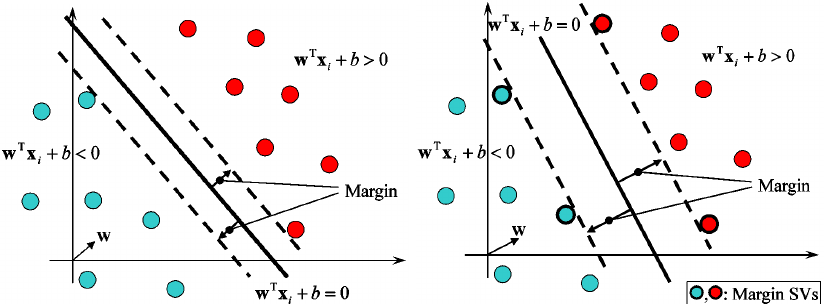
\includegraphics[scale=0.4]{svm}
			\caption{Optimal margin linear seperating hyperplane.}
		\end{figure}
		
		The SVM learning algorithm learns the parameters ($w$, $b$) of the optimal margin linear seperating hyperplane (for the data transformed to an higher dimensional feature space using the kernel trick).
		
		Maximizing the margin of the linear seperating hyperplane can be expressed as an constrained optimization problem:
		
		\begin{equation*}
			\begin{aligned}
				& \underset{w, b}{minimize}
				& & \frac{1}{2} ||w||^2 \\
				& \text{subject to}
				& & y^{(i)}(w^Tx^{(i)}+b) \geq 1, \; i = 1, \ldots, m.
			\end{aligned}
		\end{equation*}
		
		Using the langragian, the dual form of the optimization is formulated as a quadratic programming problem:
		
		\begin{equation*}
			\begin{aligned}
				& \underset{\alpha}{maximize}
				& & \Psi(\alpha) = \sum_{i=1}^{m} \alpha_i - \frac{1}{2} \sum_{i,j=1}^{m} y^{(i)} y^{(j)} \alpha_i \alpha_j \langle x^{(i)}, x^{(j)} \rangle \\
				& \text{subject to}
				& & \alpha_i \geq 0, \; i=1, \ldots, m. \\
				& & & \sum_{i=1}^{m} \alpha_i y^{(i)} = 0								
			\end{aligned}					
		\end{equation*}
		
		The parameter $w$ that characterizes the optimal margin linear seperating hyperplane is computed:
		
		\begin{equation*}
			w = \sum_{i=1}^{m} \alpha_i y^{(i)} x^{(i)}
		\end{equation*}
				
		To make the algorithm work for non-linearly seperable datasets as well as less sensitive to outliers, we reformulate the optimization (using ${\textbf l_1}$ regularization):
		
		\begin{equation}
			\label{regularised_dual_form}
			\begin{aligned}
				& \underset{\alpha}{maximize}
				& & \Psi(\alpha) = \sum_{i=1}^{m} \alpha_i - \frac{1}{2} \sum_{i,j=1}^{m} y^{(i)} y^{(j)} \alpha_i \alpha_j \langle x^{(i)}, x^{(j)} \rangle \\
				& \text{subject to}
				& & 0 \leq \alpha_i \leq C, \; i=1, \ldots, m. \\
				& & & \sum_{i=1}^{m} \alpha_i y^{(i)} = 0 \\
				& & & \text{where, \textbf{C} is the regularization parameter.}
			\end{aligned}					
		\end{equation}		
		
		The Karush-Kuhn-Tucker(KKT) conditions are necessary and sufficient for the optimal value of a positive-definite quadratic programming problem. The KKT (or convergence) conditions for the quadratic programming problem (\ref{regularised_dual_form}) for $i=1, \ldots, m$ are:
		
		\begin{equation}
			\label{kkt_conditions}
			\begin{aligned}
				\alpha_i = 0 \iff y^{(i)} (w^T x^{(i)} + b) \geq 1 \\
				\alpha_i = C \iff y^{(i)} (w^T x^{(i)} + b) \leq 1 \\
				0 < \alpha_i < C \iff y^{(i)} (w^T x^{(i)} + b) = 1 \\
			\end{aligned}
		\end{equation}

	\subsection{Modified SMO Algorithm}
			
		Let us consider the partition of training samples into $I_0 = \{i: y=1, 0 < \alpha_i < C\} \bigcup \{i: y=-1, 0 < \alpha_i < C\}$, $I_1 = \{i: y=1, \alpha_i = 0\}$, $I_2 = \{i: y=-1, \alpha_i = C\}$, $I_3 = \{i: y=1, \alpha_i = C\}$ and $I_4 = \{i: y=-1, \alpha_i = 0\}$.
	
		% Why b is not involved in computing output ?
		Let $f_i = \sum_{j=1}^{m} \alpha_j y_j \langle X_j, X_i \rangle - y_i$ denotes the error on the i\textsuperscript{th} training sample.
	
		Parameters $b_{up}$ and $b_{low}$, and the indices of corresponding training samples, $I_{up}$ and $I_{low}$ are computed:
	
		\begin{equation*}
			\begin{aligned}
				&	b_{up} = min \{ f_i : i \in I_0 \cup I_1 \cup I_2 \}, I_{up} = \argmin_{i \in I_0 \cup I_1 \cup I_2} f_i \\
				&	b_{low} = max \{ f_i : i \in I_0 \cup I_3 \cup I_4\}, I_{low} = \argmin_{i \in I_0 \cup I_3 \cup I_4} f_i \\
			\end{aligned}
		\end{equation*}
	
		The modified SMO algorithm optimizes the $\alpha_i$s associated with $b_{up}$ and $b_{low}$, i.e., $\alpha_{I_{low}}$ and $\alpha_{I_{up}}$ at each step.
	
		\begin{equation}
			\begin{aligned}
				& \alpha_2^{new} = \alpha_2^{old} - \frac{y_2 (f_1^{old} - f_2^{old})}{\eta}\\
				& \alpha_1^{new} = \alpha_1^{old} + s (\alpha_2^{old} - \alpha_2^{new})\\
			\end{aligned}
		\end{equation}		
		where variables associated with the $\alpha_i$s to be updated are represented using subscript "1" and "2", $\eta = 2 \langle X_1, X_2 \rangle - \langle X_1, X_1 \rangle - \langle X_2, X_2 \rangle$, $s = y_1 y_2$. $\alpha_1$ and $\alpha_2$ are clipped to \big[ 0, C \big].
	
		After each step, $f_i$ denoting the error on the i\textsuperscript{th} training sample is updated:
	
		\begin{equation}
			f_i^{new} = f_i^{old} + (\alpha_1^{new} - \alpha_1^{old}) y_1 \langle X_1, X_i \rangle + (\alpha_2^{new} - \alpha_2^{old}) y_2 \langle X_2, X_i \rangle.
		\end{equation}
	
		The value of the objective in (\ref{regularised_dual_form}), represented by $Dual$ is updated:
		
		\begin{equation}
			Dual^{new} = Dual^{new} - \frac{\alpha_1^{new} - \alpha_1^{old}}{y_1}(f_1^{old} - f_2^{old}) + \frac{1}{2} \eta \bigg(\frac{\alpha_1^{new} - \alpha_1^{old}}{y_1}\bigg)^2
		\end{equation}
	
		$DualityGap$, representing the difference betweeen the primal and dual objective function is calculated:
	
		\begin{equation}
			\begin{aligned}
				& DualityGap = \sum_{i=0}^{m} \alpha_i y_i f_i + \sum_{i=0}^{m} \epsilon_i \\
				& \text{where } \epsilon_i = 
					C \max (0, y_i (b-f_i))
			\end{aligned}
		\end{equation}
		$Dual$ and $DualityGap$ are used to check for convergence of the $\alpha_i$s to optimum value of (\ref{regularised_dual_form}).
	
		\begin{algorithm}[caption={Modified SMO Algorithm}]
	Initialize $\alpha_i = 0, f_i = -y_i \text{ for } i=1, \ldots, m $
	Initialize $Dual = 0$
	Calculate $b_{up}, I_{up}, b_{low}, I_{low}, DualityGap$
	Until $DualityGap \leq \tau | Dual | $
		1) Optimize $\alpha_{I_{up}}, \alpha_{I_{low}}$
		2) Update $f_i, \text{ for } i=1, \ldots, m $
		3) Calculate $b_{up}, I_{up}, b_{low}, I_{low}, DualityGap$ and Update $Dual$.
	Repeat
		\end{algorithm}
		
	\section{Parallelizing the SMO Algorithm}
		
		The entire training data set is equally partitioned into smaller subsets according to the number of processor used. Then, each of the partitioned subsets is distributed into one CPU processor. The attributes associated with each training sample, i.e., $\alpha_i$, $f_i$, are maintained locally by the processor to which the sample was distributed. A globally synchronized copy of the attributes $b$, $Dual$ and $DualityGap$ is maintained across all processors.
		
		By executing, the program of calculating $b_{up}$, $b_{low}$, $I_{up}$ and $I_{low}$ using all processors, each processor could obtain one $b_{up}$ and one $b_{low}$ as well as the associated $I_{up}$ and $I_{low}$ based on its assigned training data patterns. The global $b_{up}$ and global $b_{low}$ are, respectively the minimum value of $b_{up}$ of each processor and maximum value of $b_{low}$ of each processor. By determining the global $b_{up}$ and the global $b_{low}$, the associated $I_{up}$ and $I_{low}$ could be found out. The corresponding two $\alpha_i$, are then optimized by using any one CPU processor.
		
		Similarly, each processor computes the $DualityGap$ for a subset of training data sample. The value of $DualityGap$ on entire training data patterns is the sum of $DualityGap$ on all the processors.
		
		The computation time of sequential SMO is dominantly used for updating the $f_i$ array. By executing the program of updating $f_i$ array using all processors, each processor will update a different subset of $f_i$ array based on its training data pattern.
		
		\begin{algorithm}[caption={Parallel SMO Algorithm}]
Notation: $p$ is the total number of processes used.
$l^k$ is the subset of all training data samples indices assigned to processor k.
$\bigcup_{k=1 \rightarrow p} l^k = l$ denotes the entire set of all training data samples indices.

$f_i^k$, $\alpha_i^k$ and $i \in l^k$ denote the variables associated with samples in processor k.
$b_{up}^k$, $I_{up}^k$, $b_{low}^k$, $I_{low}^k$, $DualityGap^k$ denote the variables associated with processor k.
$f_i^k = \sum_{j=1}^{|l|} \alpha_j y_j \langle X_j, X_i \rangle - y_i$ array denotes error on training samples with processor k.
$b_{up}^k = \min\{f_i^k: i \in l^k\text{ and }i \in I_0 \cup I_1 \cup I_2\}$, $I_{up}^k$ is the index of the corresponding sample.

$b_{up}^k = \max\{f_i^k: i \in l^k\text{ and }i \in I_0 \cup I_3 \cup I_4\}$, $I_{low}^k$ is the index of the corresponding sample.
$b_{up}$, $I_{up}$, $b_{low}$, $I_{low}$, and $DualityGap$ denote the variables on entire training data.
$b_{up} = \min\{b_{up}^k\}$,$b_{low} = \max\{b_{low}^k\}$,and $I_{up}$, $I_{low}$ denote the indices of corresponding samples.
$DualityGap = \sum_{k=1}^{p} DualityGap^k$

Initialize $\alpha_i^k = 0$, $f_i^k = -y_i$, $Dual = 0$, for $i \in l^k$, $k=1,\ldots,p$
Calculate $b_{up}^k$, $I_{up}^k$, $b_{low}^k$, $I_{low}^k$ and $DualityGap^k$.

Obtain $b_{up}$, $I_{up}$, $b_{low}$, $I_{low}$ and $DualityGap$.
Until $DualityGap \leq \tau | Dual |$
1) Optimize $\alpha_{I_{up}}$,  $\alpha_{I_{low}}$
2) Update $f_i^k, i \in l^k$
3) Calculate $b_{up}^k$, $I_{up}^k$, $b_{low}^k$, $I_{low}^k$ and $DualityGap^k$.
4) Obtain $b_{up}$, $I_{up}$, $b_{low}$, $I_{low}$ and $DualityGap$, and update $Dual$.
Repeat

		\end{algorithm}

	\section{Inferences}
		The execution time of the parallelized SMO algorithm is dratically reduced for large number of training samples. However, the accuracy of prediction by the modified SMO algorithm is lower than that of the original SMO algorithm.
\pagebreak

\begin{appendices}	
	\section{Downloading and Running Source Code}
		\subsection{Downloading the Source Code}
			The source code of the parallel implementation of SMO algorithm in C using OpenMPI can be downloaded \href{https://github.com/elixir-code/HPC-Lab/raw/master/Project/SVM-OpenMPI/svm-openmpi-codes.zip}{\textbf{here}}.
			
			Please visit the github repository \href{https://github.com/elixir-code/HPC-Lab/}{\textbf{elixir-code/HPC-Lab}} for supplementary resources.
			
			\subsection{Running the Source Code}
				\begin{enumerate}
					\item Extract the zip file containing the source code.				
						\begin{lstlisting}[style=BashStyle]
$ unzip <path to downloaded source code zip>/svm-openmpi-codes.zip
						\end{lstlisting}
						
					\item Open the terminal and change the current directory to the extracted directory that contains source code.
						\begin{lstlisting}[style=BashStyle]
$ cd <path where source code zip was extracted>/svm-openmpi-codes
						\end{lstlisting}
					
					\item Compile the source code using the OpenMPI's "wrapper" compiler to generate the object file.
						\begin{lstlisting}[style=BashStyle]
$ mpicc -o <name of object file> mpisvm.c
						\end{lstlisting}
						
					\item Launch the OpenMPI parallel jobs by executing the generated object file.
						
						\begin{lstlisting}[style=BashStyle]
$ mpirun -np <number of processes> <name of generated object file>
						\end{lstlisting}	
				\end{enumerate}
	\pagebreak
	
	\section{Complete Source Code}
		\lstinputlisting[style=CStyle, caption={\textbf{mpisvm.c}}]{../svm-openmpi-codes/mpisvm.c}
		
\end{appendices}		
	
\end{document}